\documentclass{article}
\usepackage[utf8]{inputenc}
\usepackage{amsmath}
\usepackage{amssymb}
\usepackage{graphicx}
\usepackage{hyperref}
\usepackage{tikz}
\usepackage{pgfplots}
\usepackage{float}
\usepackage{listings}
\usepackage{color}
\usepackage{bbm}
\usepackage{multirow}
\usepackage{comment}

\title{Reinforcement Learning \\ Exercise 7 - Solution}
\author{Jonathan Schnitzler - st166934 \\
Eric Choquet - st160996}
\date{\today}
\begin{document}
\maketitle

\section{Linear function approximation}

\paragraph*{a)  Tabular linear function approximation}

TODO


\paragraph*{b) Update rule for Sarsa}

TODO



\section{Mountain Car}

\begin{comment}
\begin{figure}[H]
\centering
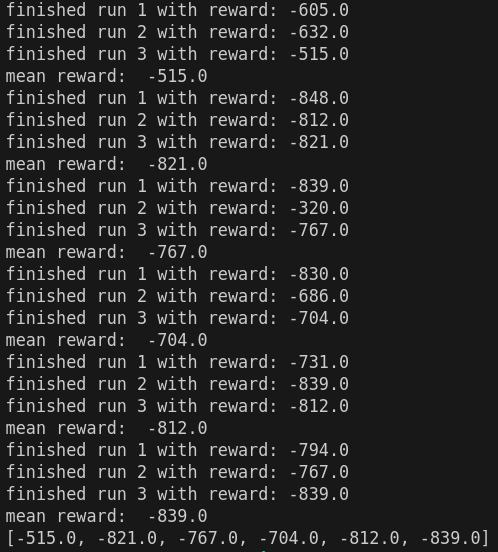
\includegraphics[width=0.5\textwidth]{images/terminal.png}
\caption{Output for Trees with \texttt{maxiter} = [10, 20, 50, 100, 200, 500]}
\label{fig:terminal}
\end{figure}
\end{comment}
TODO:

\end{document}













